\documentclass[12pt,a4paper]{scrartcl}
\usepackage[utf8]{inputenc}
\usepackage[english, russian]{babel}
\usepackage{indentfirst}
\usepackage{misccorr}
\usepackage[dvipdfmx]{graphicx}
\usepackage{amsmath}
\usepackage{multirow}
\usepackage{pgfplots}
\usepackage{parskip}
\usepackage[top=1cm, bottom=1cm, left=1cm, right=1cm]{geometry}
\pgfplotsset{compat=1.9}

\begin{document}
	\graphicspath{{py/}}
	
	\newcommand{\ms}{\mathstrut}
	\newcommand{\msp}{\hspace{0.5cm}}
	\newcommand{\al}{\alpha}
	\newcommand{\dg}{^\circ}
	\newcommand{\dif}{\mathrm{d}}
	\newcommand{\qd}[2]{^{\frac{#1}{#2}}}
	\newcommand{\qdm}[2]{^{-\frac{#1}{#2}}}
	\newcommand{\lm}[2]{\underset{#1 \rightarrow #2}{\lim}}
	\newcommand{\sfrac}[2]{\dfrac{\strut #1}{\strut #2}}
	\newcommand{\equal}[1]{\overset{(#1)}{=}}
	\newcommand{\linevdots}{\ \raisebox{-.08\height}{\vdots}\ }
	\newcommand{\linecvdots}{\ \raisebox{-.08\height}{\vdots}\hspace{-0.13cm}\raisebox{.15\height}{\cancel{\phantom{a}}\hspace{0.06cm}}}
	\newcommand{\combox}[1]{\ms \msp \msp \begin{minipage}{0.95\linewidth}
			#1
	\end{minipage}}
	
	\newtheorem{pr}{Задача}
	\newtheorem{ex}{Пример}
	\newtheorem{dfn}{Def}
	\newtheorem{theorem}{Th}
	
	\newenvironment{slv}{\ms \msp \textit{Решение:}}{}
	\newenvironment{proof}{\ms \msp \textit{Доказательство: }}{\hfill $\square$}
	
	\begin{titlepage}
		
		\vspace*{\fill}
		
		\begin{center}
			
\includegraphics[scale=0.8]{MIPT.png}
			\\[0.7cm]\Huge Московский Физико-Технический Институт\\(национальный исследовательский университет)
			\\[2cm]\LARGE Отчет по эксперименту
			\\[0.5cm]\noindent\rule{\textwidth}{1pt}
			\\\Huge\textbf{Определение удельного заряда электрона}
			\\[-0.5cm]\noindent\rule{\textwidth}{1pt}
		\end{center}
		
		\begin{flushleft}
			\textit{Работа №3.3.1; дата: 18.11.22}\hfill\textit{Семестр: 3}
		\end{flushleft}
		
		\vspace*{\fill}
		
		\begin{flushleft}
			Выполнил: \hspace{\fill} Группа:
			\\Кошелев Александр \hspace{\fill} Б05-105
		\end{flushleft}
	\end{titlepage}
	
	%Страница 2
	
	\begin{flushleft}
		\footnotesize{Определение удельного заряда электрона} \hspace{\fill} \footnotesize{2}
		\\[-0.3cm]\noindent\rule{\textwidth}{0.3pt}
	\end{flushleft}
	
	\part*{А. Метод магнитной фокусировки}	
	
	\section{Аннотация}
	
	\textbf{Цель работы: }
	
	Определение значения магнитных полей, при которых происходит фокусировка электронного пучка, и по результатам измерений считать удельный заряд электрона $e/m$.	
	
	\textbf{Схема установки:}
	\begin{center}
		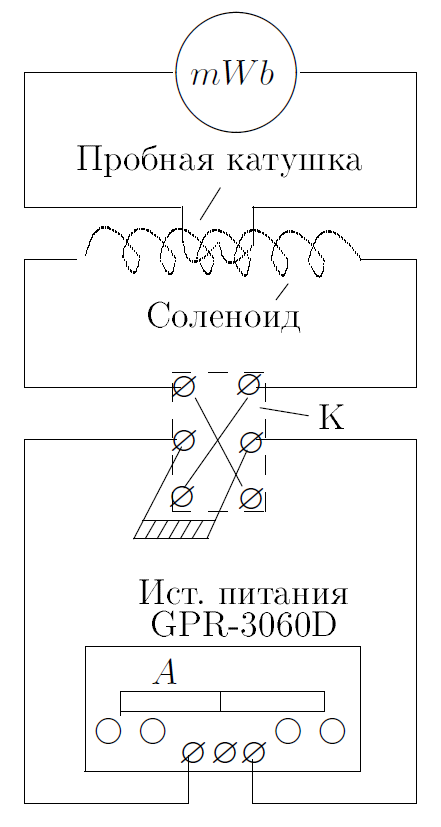
\includegraphics[scale=0.4]{PIC_1.png}
		\\\textbf{Рис. 1:} Схема установки
	\end{center}
	
		Основной частью установки является электронный осциллограф, трубка которого вынута и установлена в длинном соленоиде, создающим магнитное поле. Напряжение на отклоняющие пластины и питание подводятся к трубке многожильным кабелем.

Пучок электронов, вылетающих из катода с разными скоростями, ускоряется анодным напряжением. Пропустив пучок сквозь две узкие диафрагмы, можно выделить электроны с практически одинаковой продольной скоростью. Небольшое переменное напряжение, поступающее с клеммы "Контрольный сигнал" осциллографа на отклоняющие пластины, изменяет только поперечную составляющую скорости. При увеличении магнитного поля линия на экране стягивается в точку, а затем снова удлиняется. 

Магнитное поле создается постоянным током, величина которого регулируется ручками источника питания и измеряется амперметром. Ключ служит для изменения направления поля в соленоиде.

Величина магнитного поля определяется с помощью милливеберметра.

На точность результатов может влиять внешнее магнитное поле, особенно продольное. 

Измерения магнитного поля с помощью милливеберметра обычно проводятся в предварительных опыта: при отключении ключа устанавливается связь между силой тока и индукцией магнитного поля в соленоиде.

	\textbf{В работе используются:}
	
	Электронно-лучевая трубка и блок питания к ней; источник постоянного тока; соленоид; электростатический вольтметр; милливеберметр; ключи.

\newpage
	%Страница 3
	
	\begin{flushleft}
		\footnotesize{Определение удельного заряда электрона} \hspace{\fill} \footnotesize{3}
		\\[-0.3cm]\noindent\rule{\textwidth}{0.3pt}
	\end{flushleft}

\section{Теоретическая справка}

	\begin{center}
		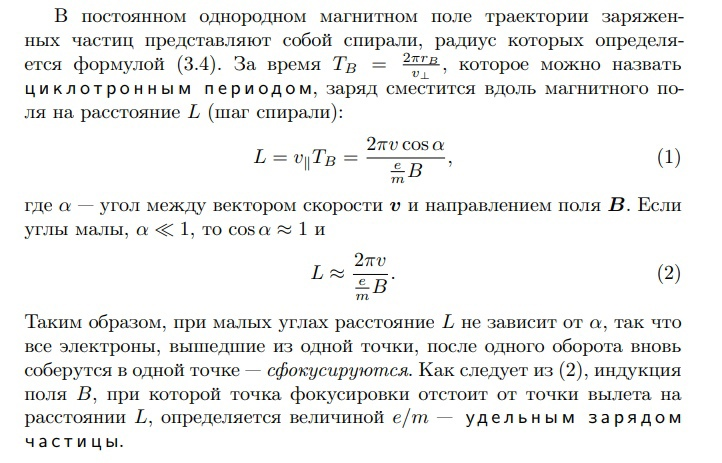
\includegraphics[scale=0.7]{THEO_1.jpg}
	\end{center}
	
	\begin{center}
		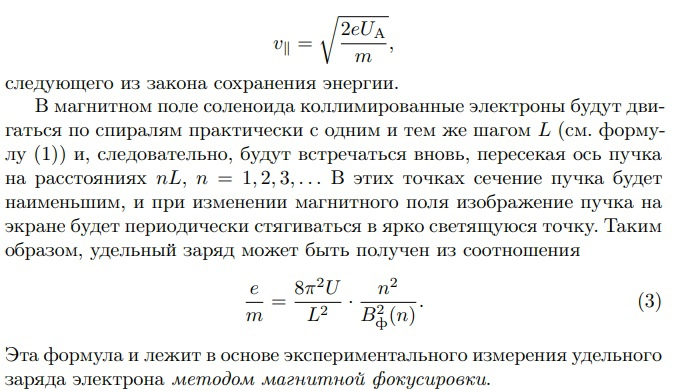
\includegraphics[scale=0.7]{THEO_2.jpg}
	\end{center}
	
	\newpage
	%Страница 4
	
	\begin{flushleft}
		\footnotesize{Определение удельного заряда электрона} \hspace{\fill} \footnotesize{4}
		\\[-0.3cm]\noindent\rule{\textwidth}{0.3pt}
	\end{flushleft}
	
	\section{Ход работы}
	
	Занесем в таблицу параметры установки.
\begin{center}
\begin{tabular}{|c|c|}
\hline
Величина & Значение  \\ \hline
$V$, кВ & 0,78  \\ \hline
$l$, м & 0,265  \\ \hline
$SN$, м$^2$ & 0,3  \\ \hline
\end{tabular}\\
\textbf{Таблица 1.} Параметры установки.
\end{center}
Для начала стоит определить связь между индукцией $B$ магнитного поля в соленоиде и током $I$ через обмотки магнита. Для этого снимем зависимость магнитного потока $\Phi = BSN$ от тока $I$.

  \begin{center}
  \begin{tabular}{|c|c|c|c|}
\hline
$I$, A & $\sigma_I$, А & $\Phi$, мВб & $\sigma_{\Phi}$, мВб \\ \hline
0,26 & 0,01 & 0,4 & 0,1 \\ \hline
0,41 & 0,01 & 0,6 & 0,1 \\ \hline
0,79 & 0,01 & 1,2 & 0,1 \\ \hline
1,01 & 0,01 & 1,4 & 0,1 \\ \hline
1,49 & 0,01 & 2,0 & 0,1 \\ \hline
2,28 & 0,01 & 3,1 & 0,1 \\ \hline
2,54 & 0,01 & 3,5 & 0,1 \\ \hline
3,06 & 0,01 & 4,2 & 0,1 \\ \hline
3,53 & 0,01 & 4,9 & 0,1 \\ \hline
\end{tabular}\\
  \textbf{Табл. 2:} Зависимость $\Phi (I)$ в прямом направлении.\\
  \end{center}
  
    \begin{center}
    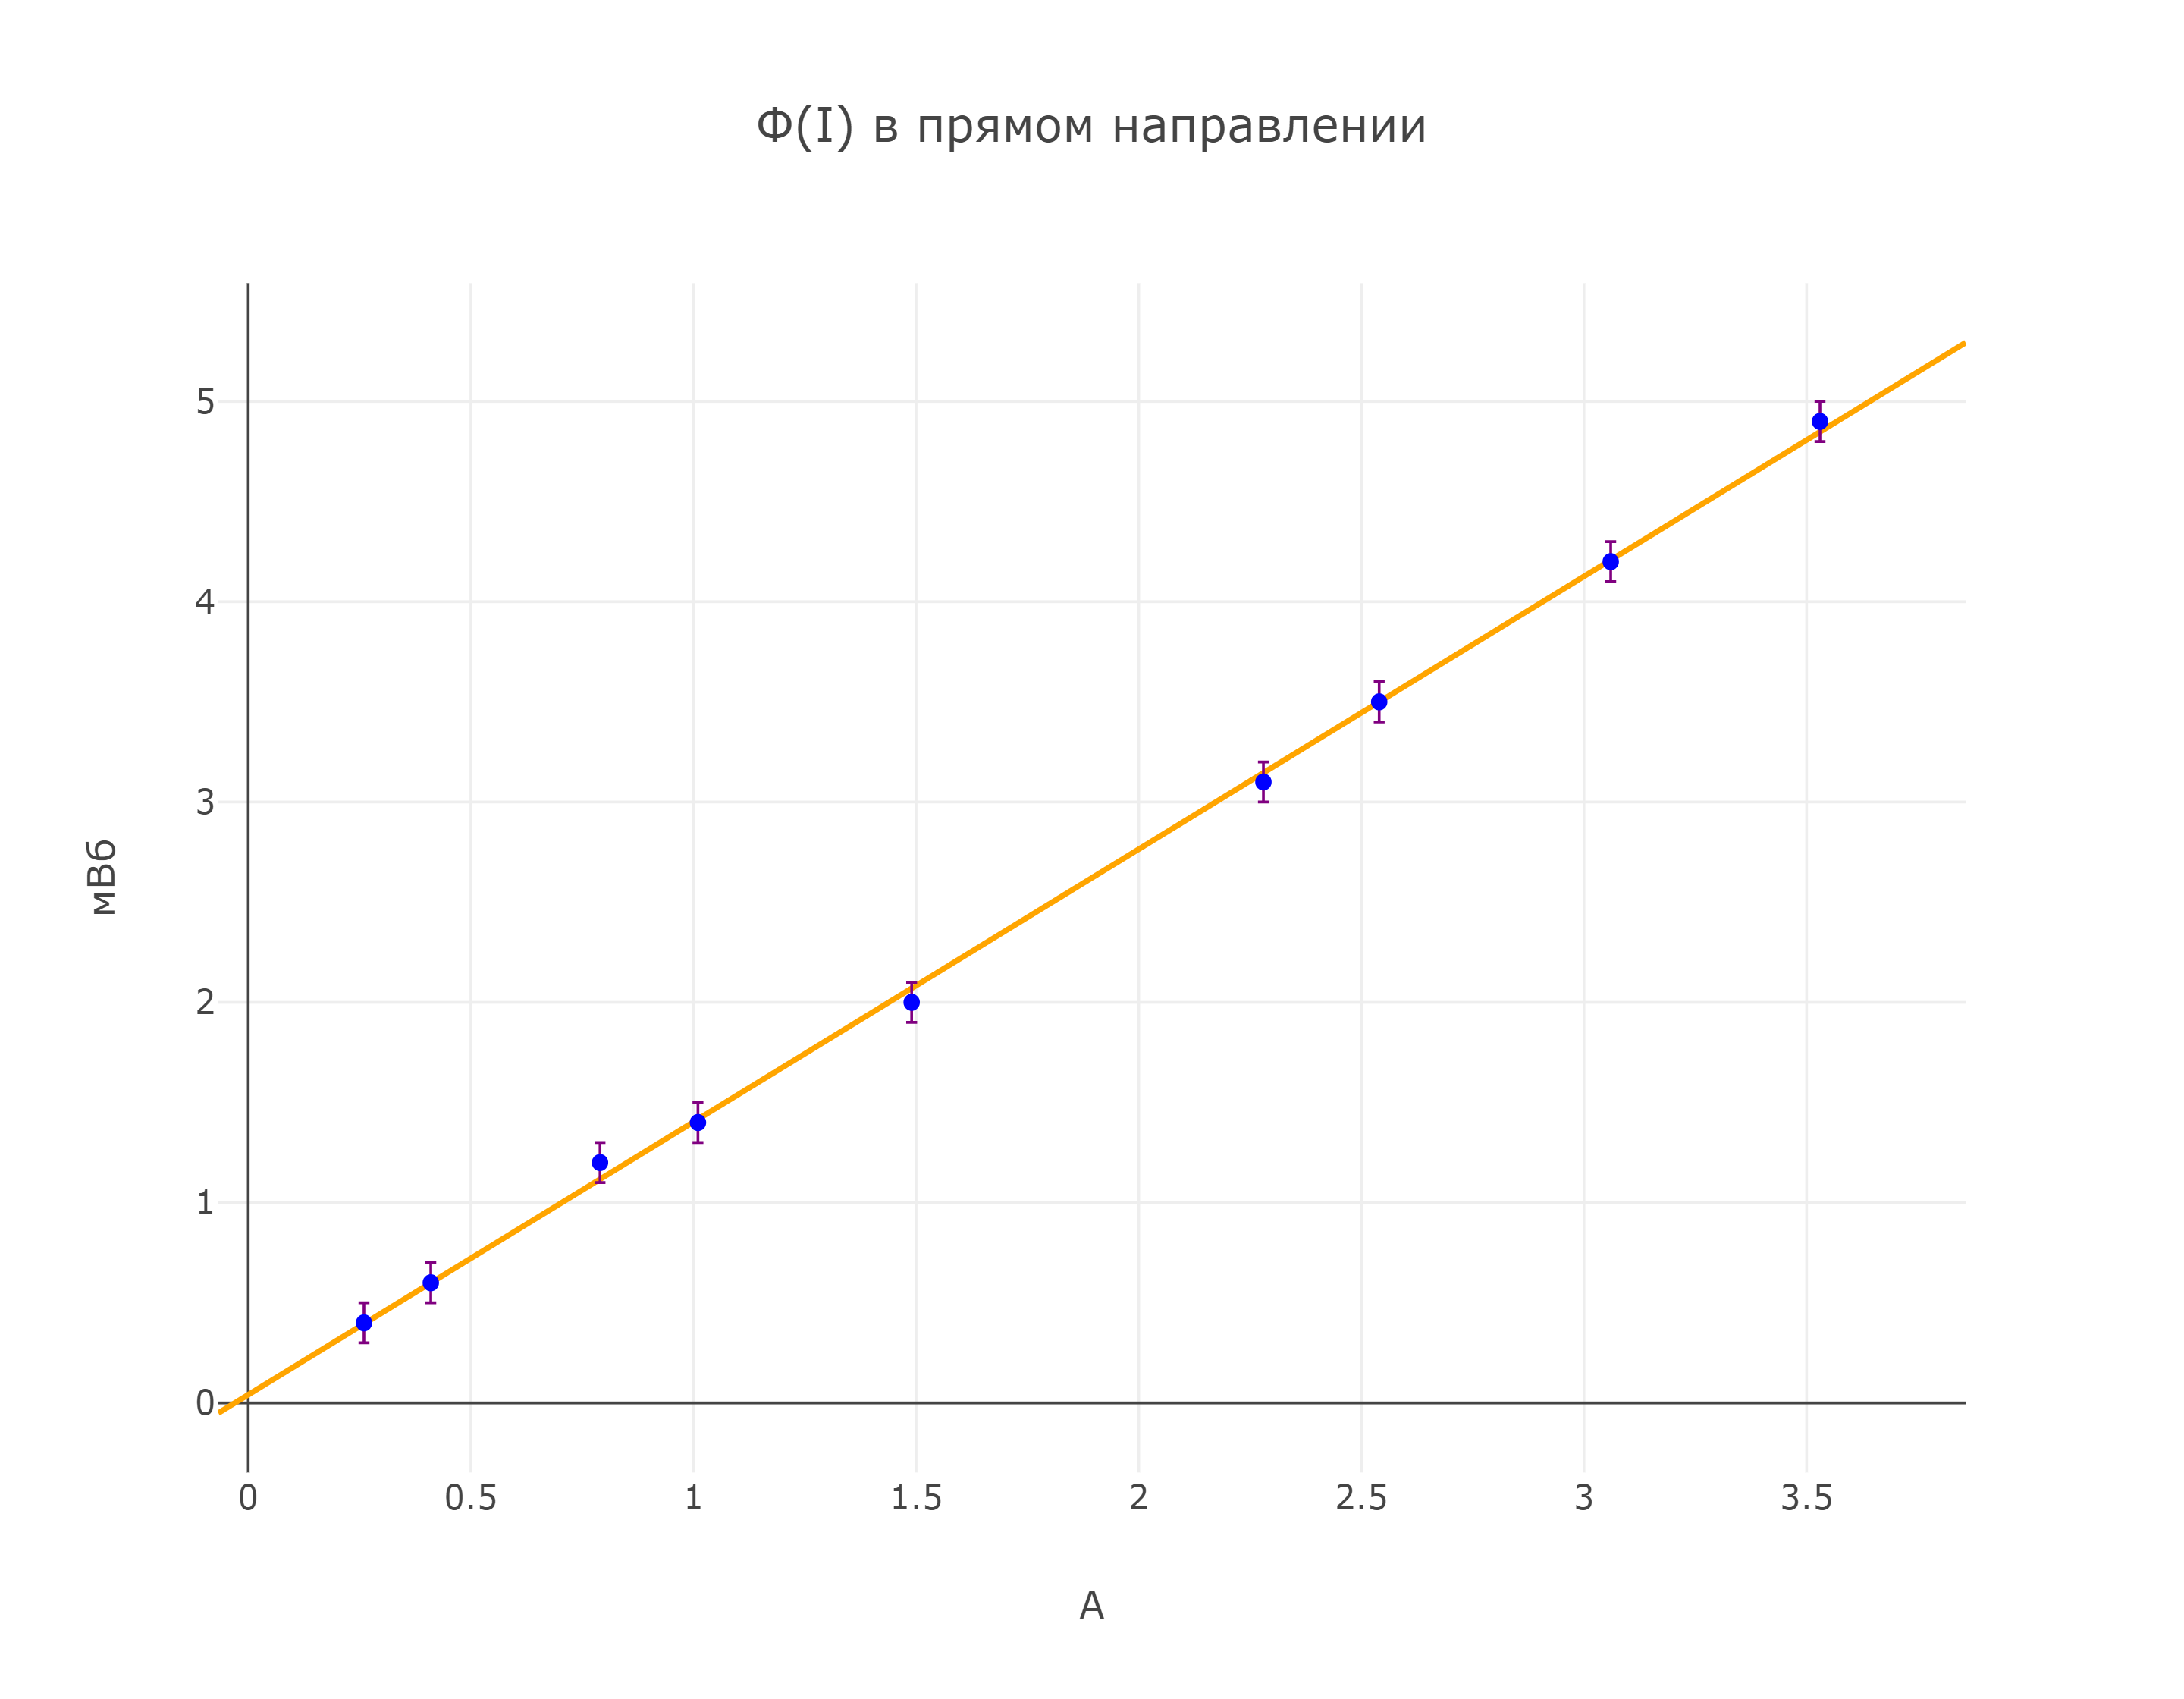
\includegraphics[width = 0.7\textwidth]{PIC_2.png}\\
  \textbf{Рис. 2:} $\Phi (I)$ в прямом направлении.
  \end{center}
  
	\newpage
	%Страница 5
	
	\begin{flushleft}
		\footnotesize{Определение удельного заряда электрона} \hspace{\fill} \footnotesize{5}
		\\[-0.3cm]\noindent\rule{\textwidth}{0.3pt}
	\end{flushleft}  
  
  \begin{center}
\begin{tabular}{|c|c|c|c|}
\hline
$I$, A & $\sigma_I$, А & $\Phi$, мВб & $\sigma_{\Phi}$, мВб \\ \hline
0,26 & 0,01 & 0,3 & 0,1 \\ \hline
0,41 & 0,01 & 0,5 & 0,1 \\ \hline
0,79 & 0,01 & 1,1 & 0,1 \\ \hline
1,01 & 0,01 & 1,3 & 0,1 \\ \hline
1,49 & 0,01 & 2,0 & 0,1 \\ \hline
2,28 & 0,01 & 3,2 & 0,1 \\ \hline
2,54 & 0,01 & 3,5 & 0,1 \\ \hline
3,06 & 0,01 & 4,2 & 0,1 \\ \hline
3,53 & 0,01 & 4,8 & 0,1 \\ \hline
\end{tabular}\\
\textbf{Табл. 3:} Зависимость $\Phi (I)$ в обратном направлении.
  \end{center} 
 \begin{center}
    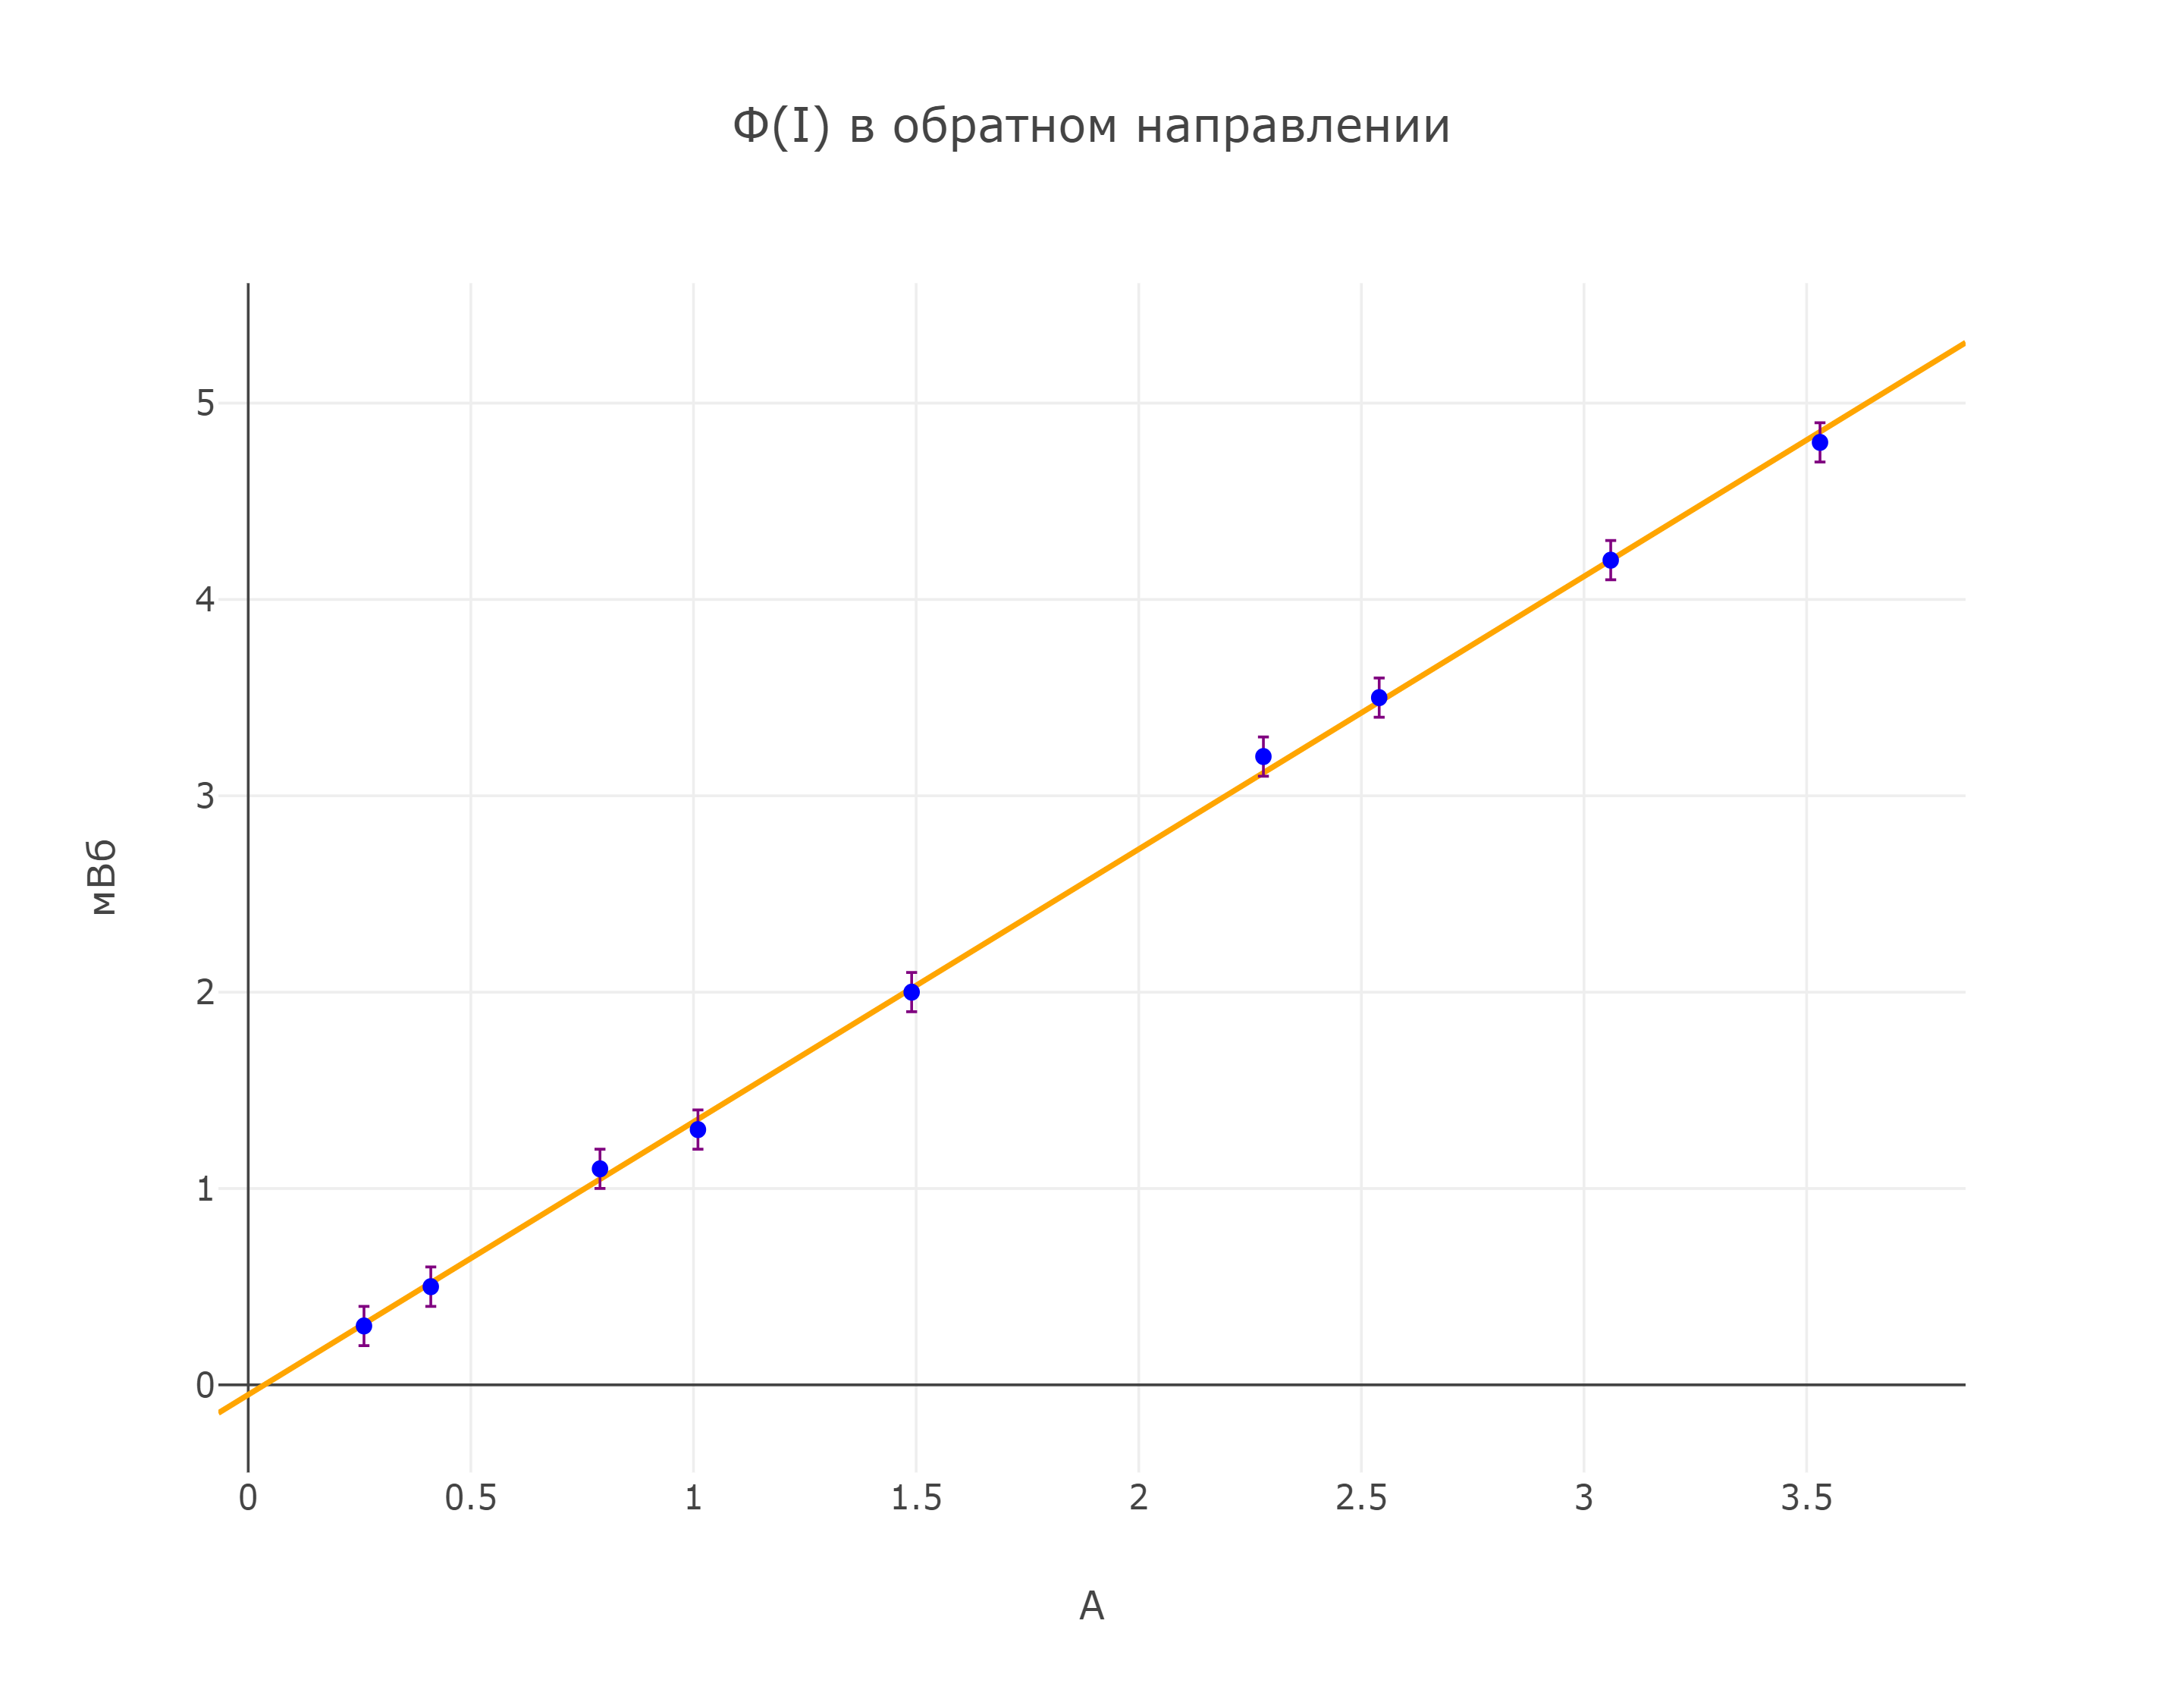
\includegraphics[width = 0.7\textwidth]{PIC_3.png}\\
  \textbf{Рис. 3:} $\Phi (I)$ в обратном направлении.
  \end{center}  
  
Графики $\text{Ф}(I)$ подчиняются линейным зависимостям с коэффициентами $\alpha_1 = (1,36 \pm 0,03) \frac{\text{мВб}}{\text{А}}$ и $\alpha_2 = (1,39 \pm 0,03) \frac{\text{мВб}}{\text{А}}$.Теперь будем увеличивать постепенно ток и найдем ток при каждом фокусе, так как мы знаем зависимость $\Phi = \Phi(I)$ для каждого направления, то мы можем определить зависимость $B_{\Phi} = f(n)$. При этом можно считать, что $\sigma_{B_{\text{Ф}}} = B_{\text{Ф}} \cdot \varepsilon_{alpha}$
\begin{center}
\begin{tabular}{|c|c|c|c|c|c|c|c|c|c|}
\hline
\multicolumn{5}{|c|}{В прямом направлении} & \multicolumn{5}{c|}{В обратном направлении} \\ \hline
n & $I_{\Phi}$, A & $\sigma_{I_{\Phi}}$, A & $B_{\Phi}$, мТл & $\sigma_{B_{\Phi}}$, мТл & n & $I_{\Phi}$, A & $\sigma_{I_{\Phi}}$, A & $B_{\Phi}$, мТл & $\sigma_{B_{\Phi}}$, мТл \\ \hline
1 & 0,55 & 0,01 & 2,63 & 0,26 & 1 & 0,55 & 0,01 & 2,38 & 0,25 \\ \hline
2 & 1,09 & 0,01 & 5,07 & 0,31 & 2 & 1,09 & 0,01 & 4,88 & 0,30 \\ \hline
3 & 1,65 & 0,01 & 7,61 & 0,37 & 3 & 1,68 & 0,01 & 7,62 & 0,36 \\ \hline
4 & 2,15 & 0,01 & 9,88 & 0,42 & 4 & 2,28 & 0,01 & 10,40 & 0,42 \\ \hline
5 & 2,69 & 0,01 & 12,33 & 0,47 & 5 & 2,79 & 0,01 & 12,76 & 0,47 \\ \hline
\end{tabular}\\
\textbf{Табл. 4:} Зависимость $B_{\Phi} = f(I)$.
\end{center}  
  
 	\newpage
	%Страница 6
	
	\begin{flushleft}
		\footnotesize{Определение удельного заряда электрона} \hspace{\fill} \footnotesize{6}
		\\[-0.3cm]\noindent\rule{\textwidth}{0.3pt}
	\end{flushleft} 
  
\begin{center}
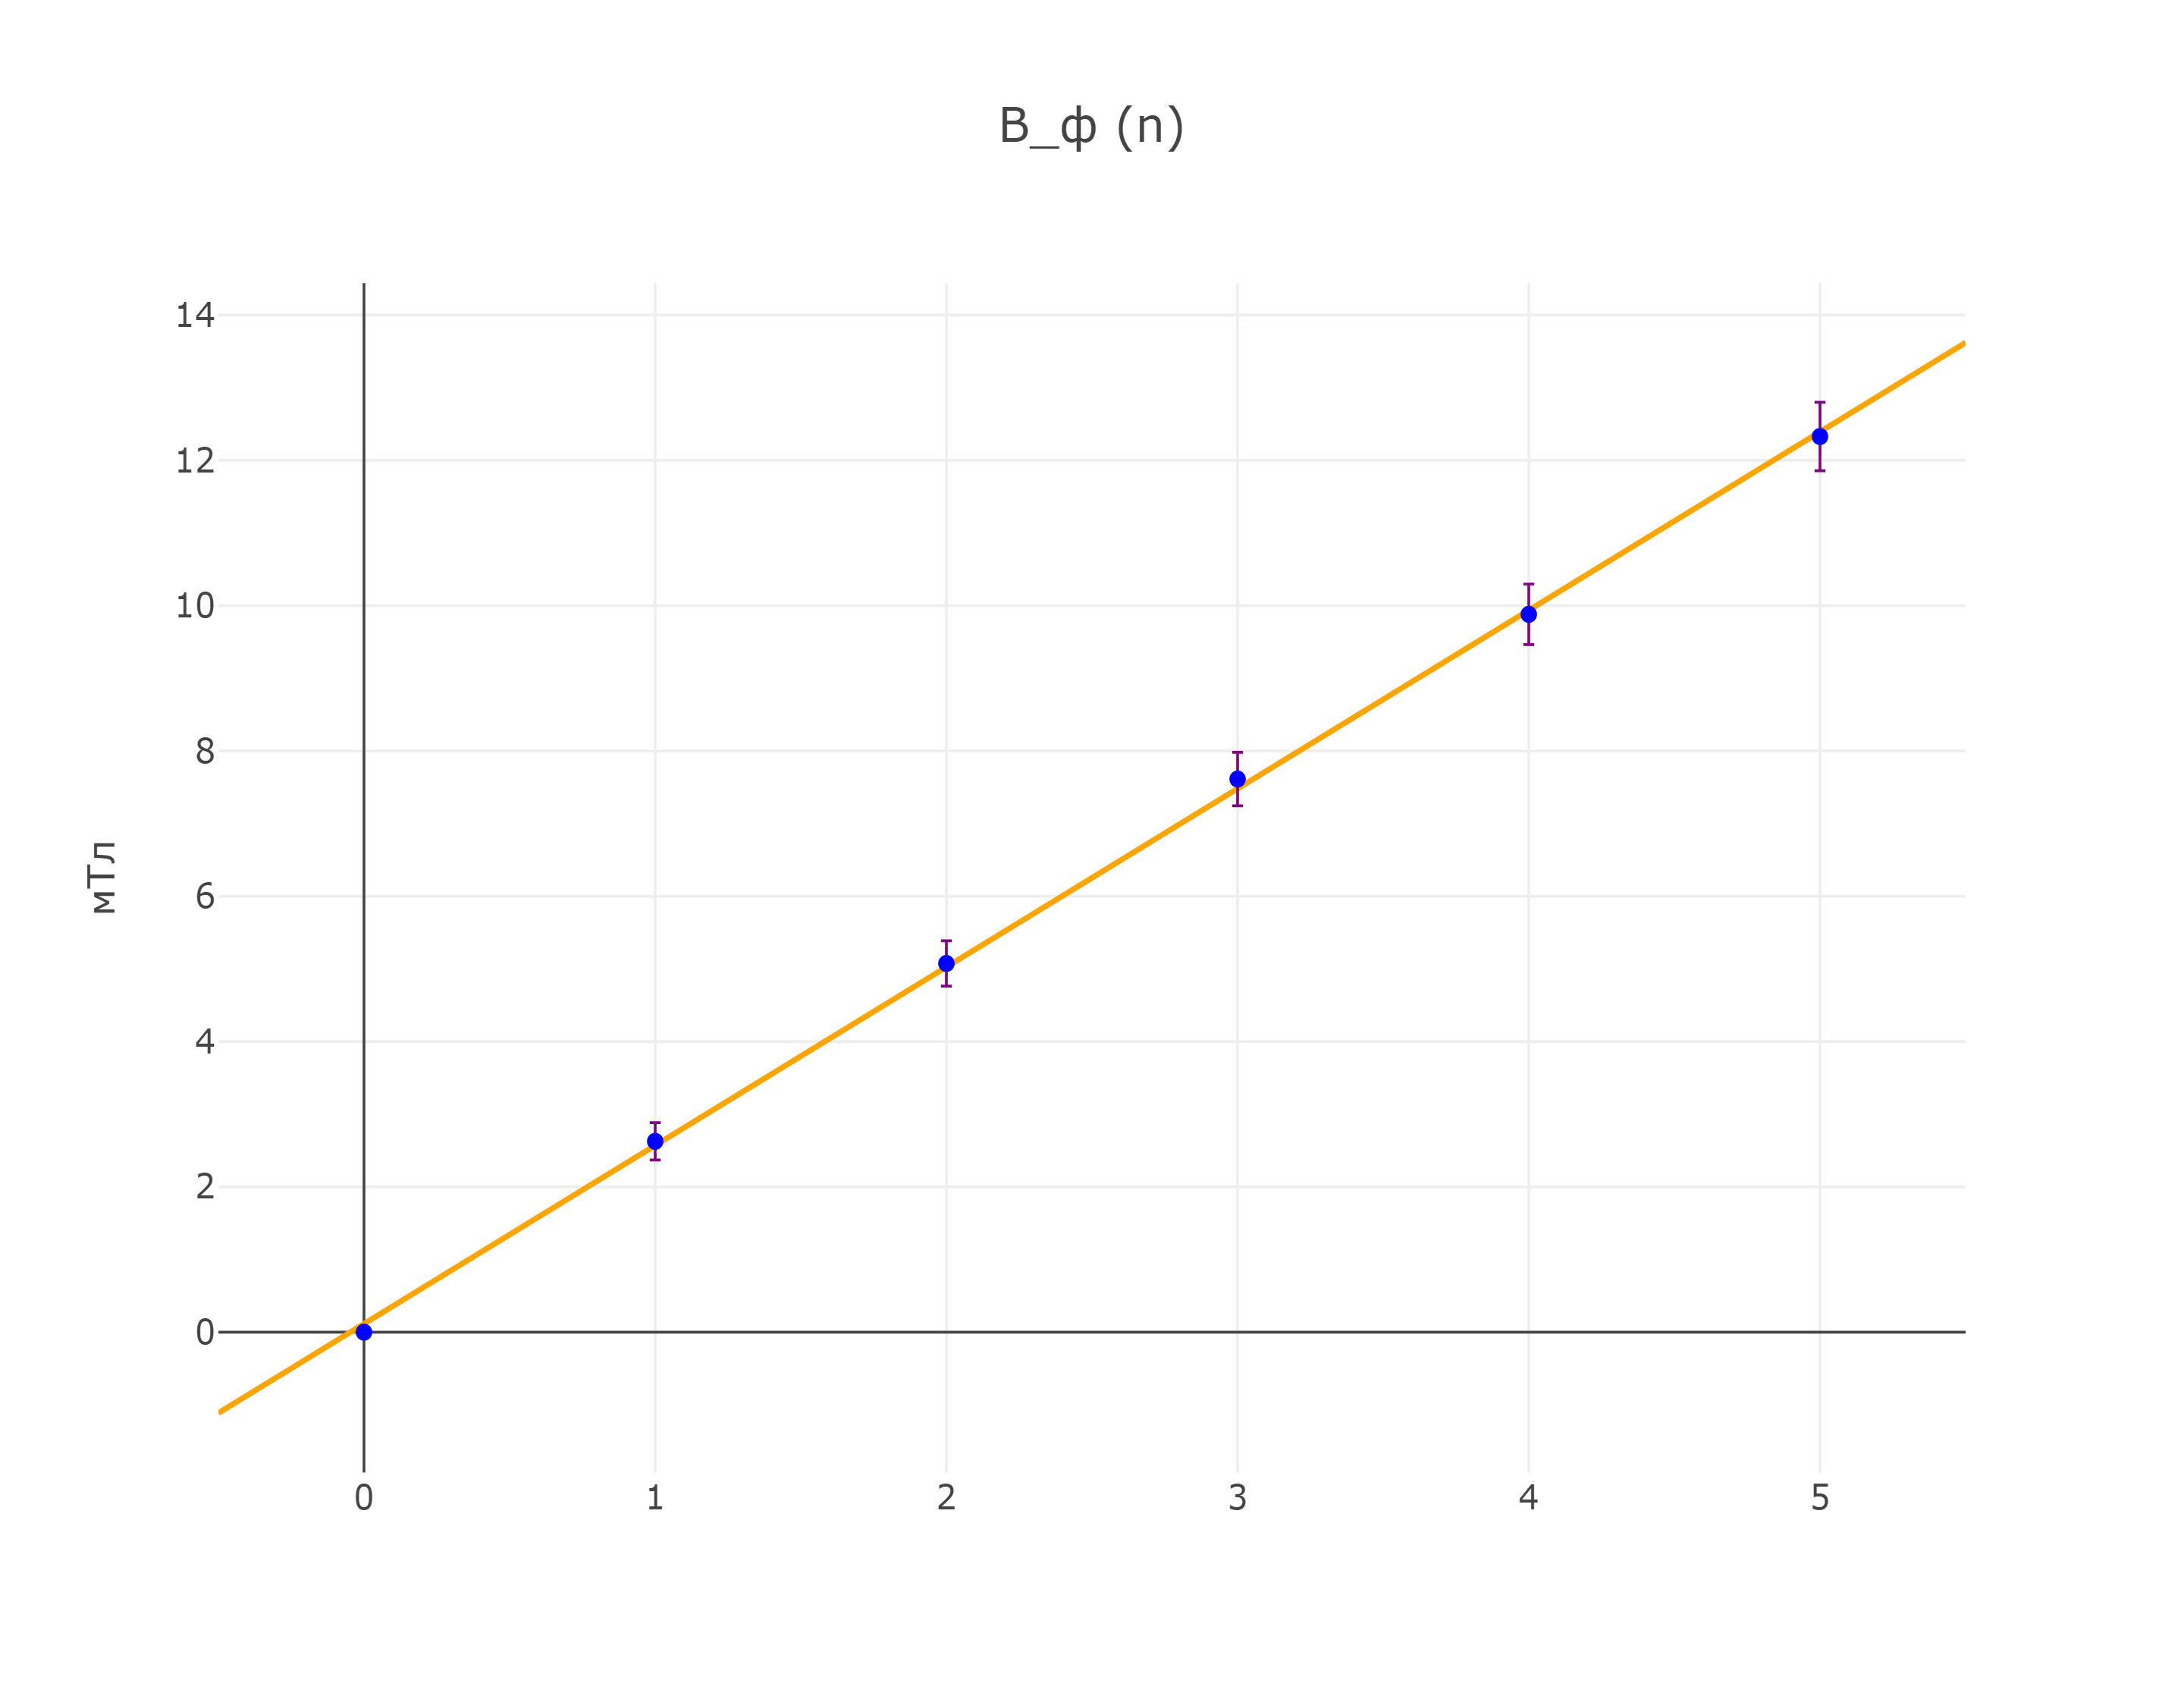
\includegraphics[width = 0.8\textwidth]{PIC_4.png}\\
\textbf{Рис. 4: } $B_{\Phi} = f(I)$ в прямом направлении.
\end{center}
\begin{center}
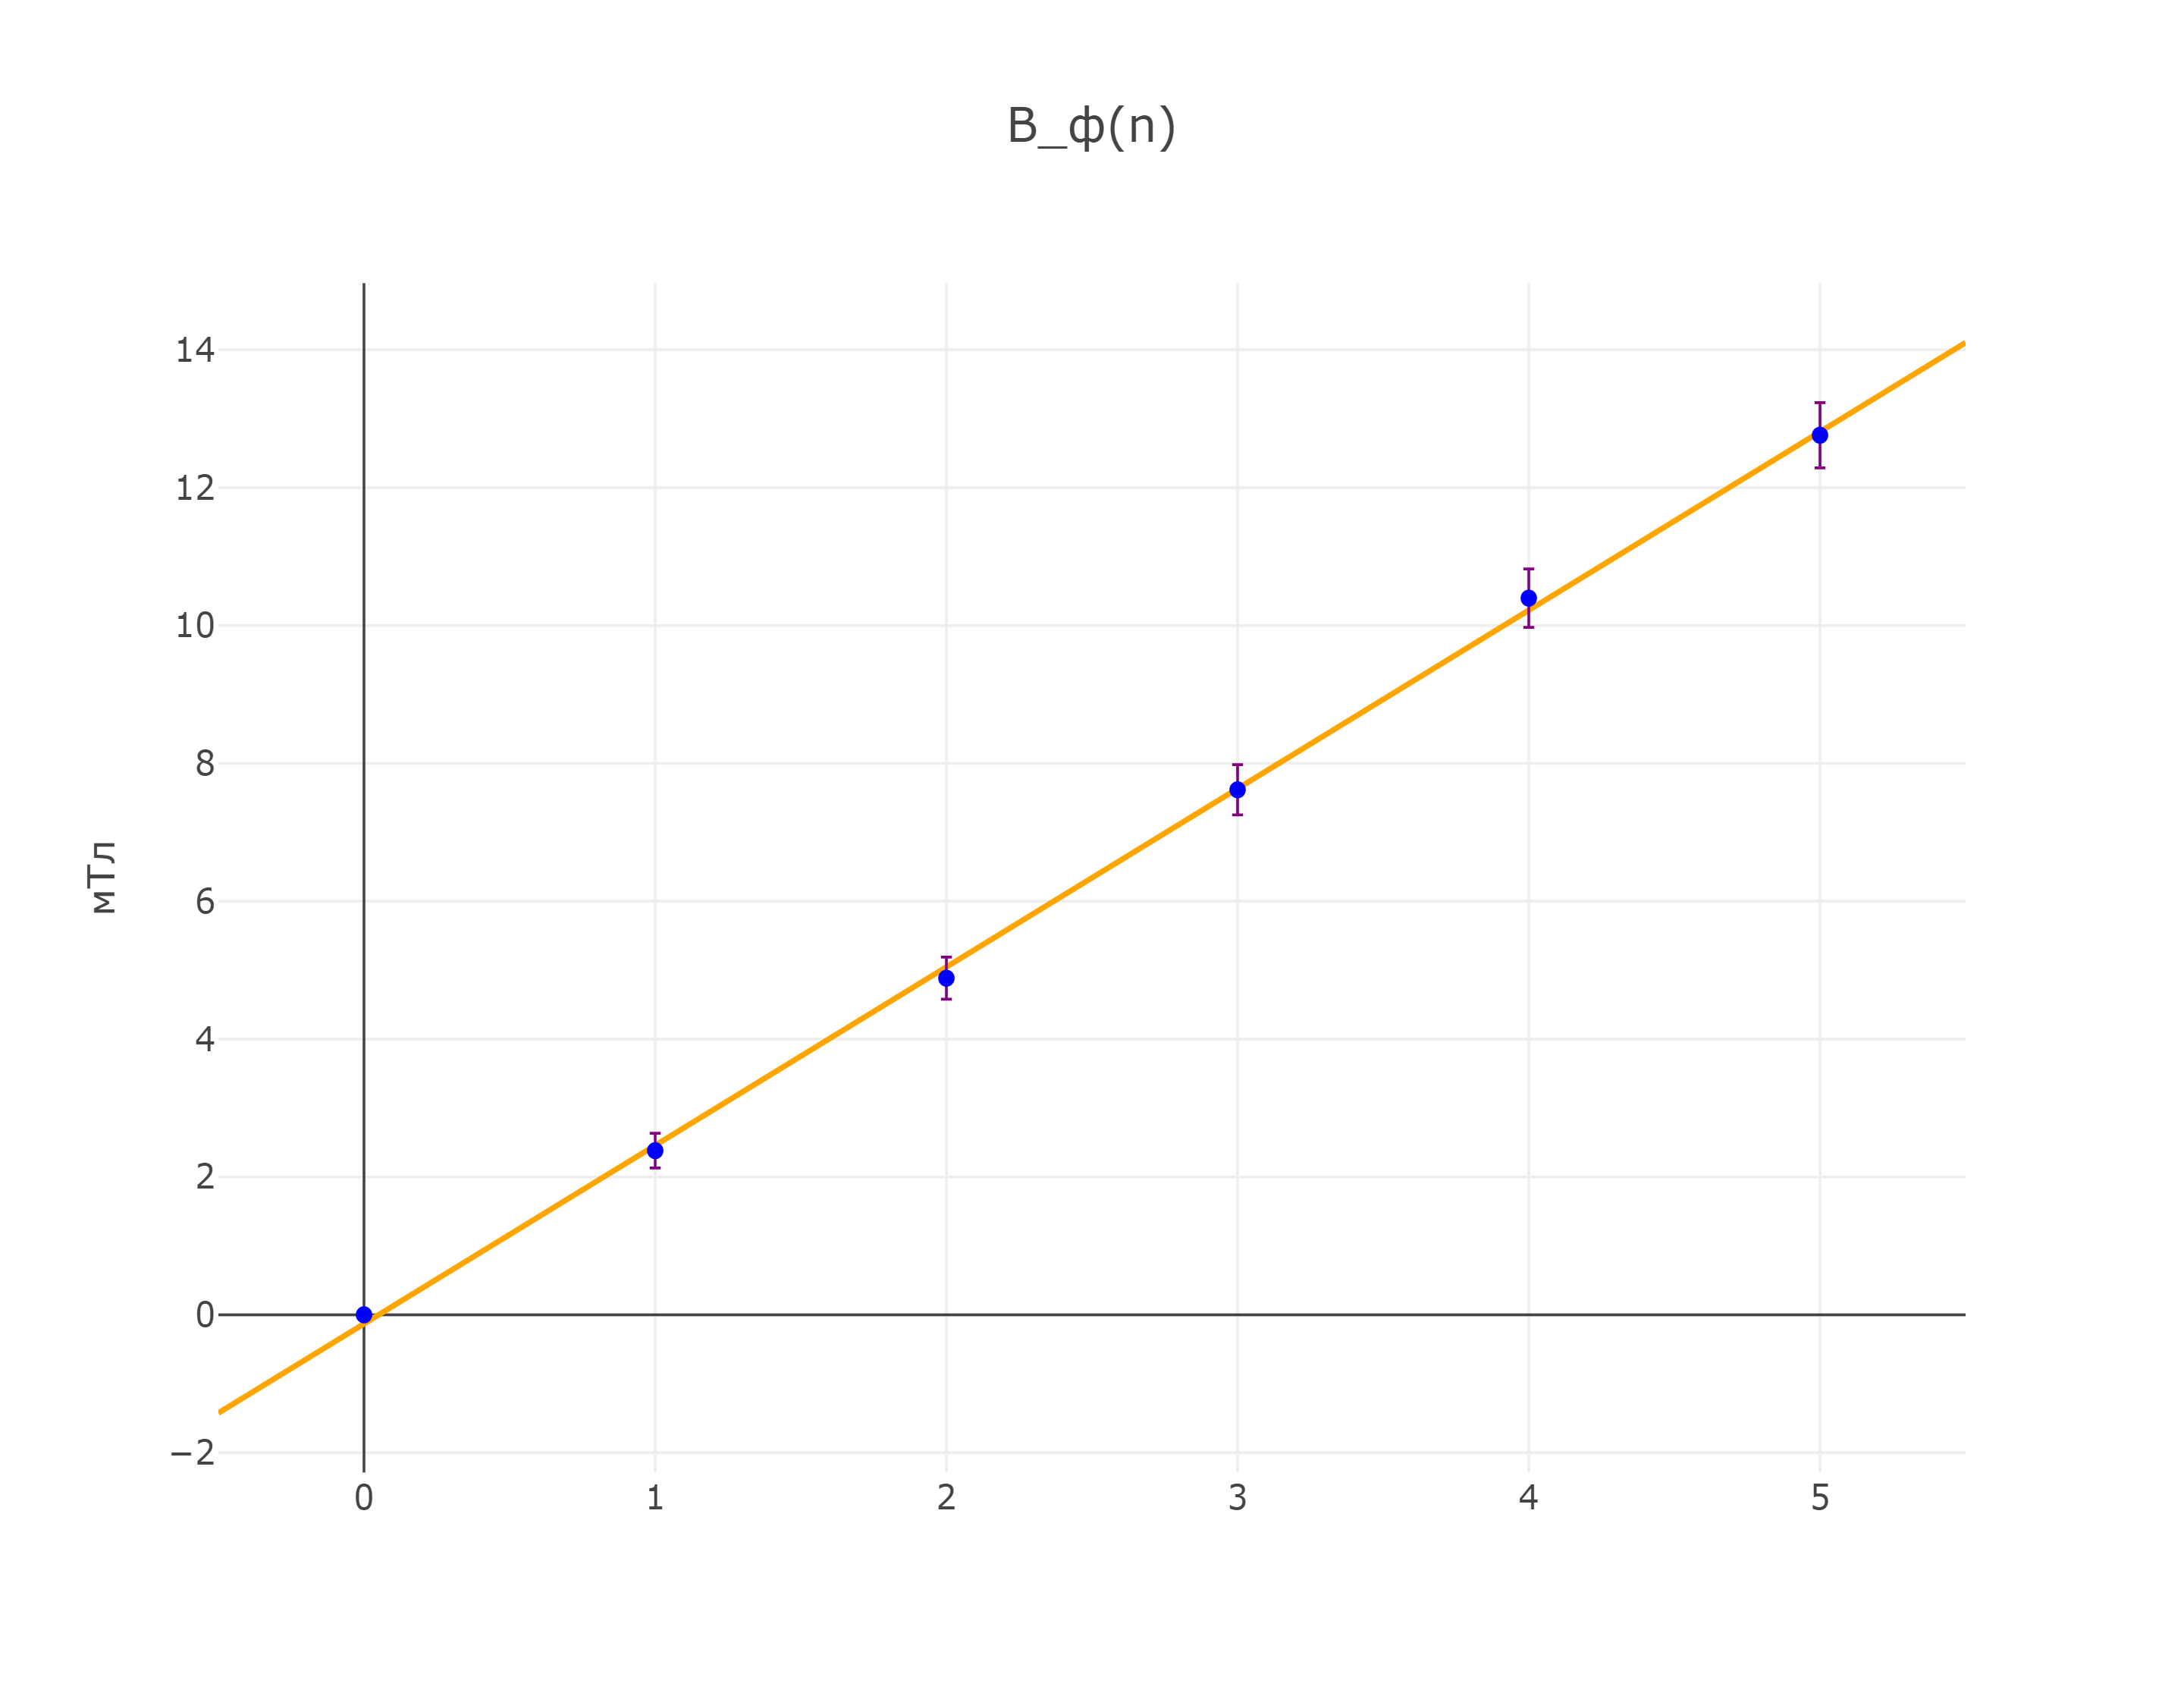
\includegraphics[width = 0.8\textwidth]{PIC_5.png}\\
\textbf{Рис. 5: } $B_{\Phi} = f(I)$ в обратном направлении.
\end{center}
Угловые коэффициенты $k_1 = 2,46 \pm 0,05 \ \text{мТл}, k_2 = 2,59 \pm 0,07 \ \text{мТл}.$ Угловые коэффициенты совпадают в рамках погрешности. Возьмем усредненное значение $k = 2,54 \pm 0,13 \ \text{мТл}$.

 	\newpage
	%Страница 7
	
	\begin{flushleft}
		\footnotesize{Определение удельного заряда электрона} \hspace{\fill} \footnotesize{7}
		\\[-0.3cm]\noindent\rule{\textwidth}{0.3pt}
	\end{flushleft} 

 В итоге, подставив в формулу $(3)$ мы получаем, что 
\[\dfrac{e}{m} = \left(1,4 \pm 0,2\right) \cdot 10^{11} \text{Кл}/\text{кг}, \varepsilon = 0,1\]  
  
\section{Выводы}  
  
В данной работе мы нашли знаечения магнитных полей при которых происходит фокусировка электронного пучка и по ним рассчитали значение удельного заряда и получили: $e/m = (1,4 \pm 0,2) \cdot 10^{11} \text{Кл}/\text{кг}$. Это значение  близко к реальному $e/m = 1,76 \cdot 10^{11} \text{Кл}/\text{кг}$

	\part*{B. Метод магнетрона}	
	\setcounter{section}{0}
	\section{Аннотация}
	
		\textbf{Цель работы: }
	
Исследование зависимости анодного тока от тока, протекающего через соленоид при различных напряжениях на аноде лампы и по результатам измерений рассчитать удельный заряд электрона $e/m$.	
	
	\textbf{Схема установки:}
	\begin{center}
		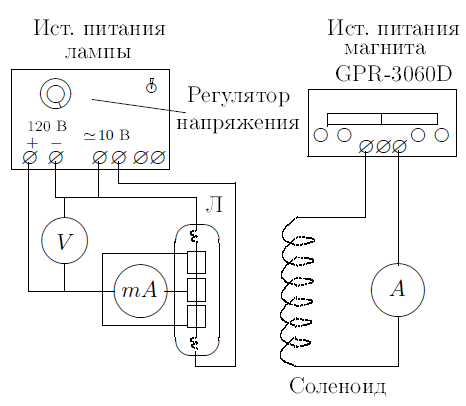
\includegraphics[scale=0.7]{PIC_6.png}
		\\\textbf{Рис. 6:} Схема установки
	\end{center}
	
		Два крайних цилиндра изолированы от среднего небольшими зазорами и используются для устранения краевых эффектов на торцах среднего цилиндра, ток с которого используется при измерениях. В качестве катода используется тонкая вольфрамовая проволока. Катод разогревается переменным током, отбираемым от стабилизированного источника питания. 

С этого же источника на анод лампы подается напряжение, регулируемое с помощью потенциометра и измеряемое вольтметром.

Индукция магнитного поля в соленоиде рассчитывается по току $I_m$, протекающему через обмотку соленоида. Коэффициент пропорциональности между ними указан в установке.

Лампа закреплена в соленоиде. Магнитное поле в соленоиде создается постоянным током, сила которого регулируется ручками источника питания и измеряется амперметром.

	\textbf{В работе используются:}
	
	Электронная лампа с цилиндрическим анодом; соленоид; источники питания лампы и соленоида; вольтметр постоянного тока; миллиамперметр, амперметр.
	
\newpage
	%Страница 8
	
	\begin{flushleft}
		\footnotesize{Определение удельного заряда электрона} \hspace{\fill} \footnotesize{8}
		\\[-0.3cm]\noindent\rule{\textwidth}{0.3pt}
	\end{flushleft}

\section{Теоретическая справка}	

\begin{center}
    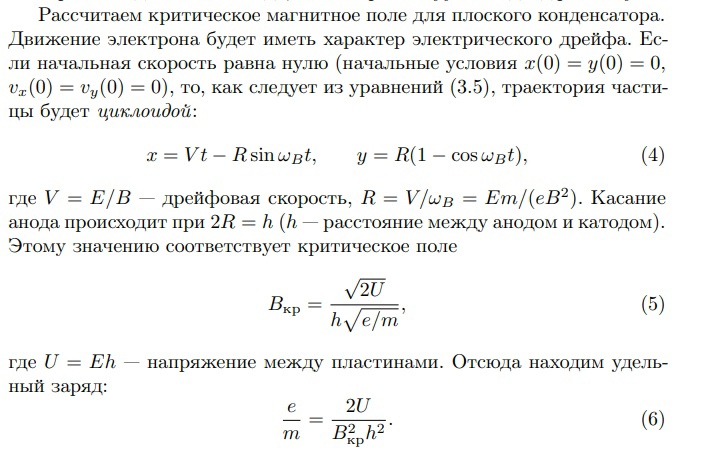
\includegraphics[scale=0.7]{THEO_3.jpg}\\
  \end{center}
  
Здесь удельный заряд электрона определяется по формуле

$$\dfrac{e}{m_e} = \dfrac{8V_a}{B_{\text{кр}}^2r_a^2}$$

где $V_a$ - анодное напряжение, $B_{\text{кр}}$ - критическое поле, $r_a$ - радиус анода.
	
\section{Ход работы}

Запишем параметры установки в таблицу
\begin{center}
\begin{tabular}{|c|c|c|}
\hline
Величина & Значение  \\ \hline
$K$, Тл/A & $2,8 \cdot 10^{-2}$  \\ \hline
$r_a$, мм & 12  \\ \hline
\end{tabular}\\
\textbf{Табл. 5:} Параметры установки
\end{center}	
	
Снимем зависимость анодного тока от тока через соленоид для различных значений $V_a$. $\sigma_{I_m}=1 \text{у.е.} = 4 \text{мА}$, $\sigma_{I_a}=1 \text{у.е.} = 4 \text{мкА}$

	\newpage
	%Страница 9
	
	\begin{flushleft}
		\footnotesize{Определение удельного заряда электрона} \hspace{\fill} \footnotesize{9}
		\\[-0.3cm]\noindent\rule{\textwidth}{0.3pt}
	\end{flushleft}
	
	\begin{figure}[h]
	\begin{minipage}{0.5\linewidth}
	\begin{center}
\begin{tabular}{|c|c|}
\hline
$I_m$, у.е. & $I_a$, у.е. \\ \hline
0 & 104  \\ \hline
20 & 104  \\ \hline
23 & 99  \\ \hline
25 & 100  \\ \hline
27 & 98  \\ \hline
28 & 92  \\ \hline
30 & 87  \\ \hline
34 & 80  \\ \hline
38 & 64  \\ \hline
40 & 55  \\ \hline
43 & 37  \\ \hline
66 & 0  \\ \hline
75 & 0  \\ \hline
\end{tabular}\\
\textbf{Табл. 6:} Зависимость $I_a(B)$ для $V_a = 70 $ В.
\end{center}
	\end{minipage}
	\begin{minipage}{0.5\linewidth}
	\begin{center}
\begin{tabular}{|c|c|}
\hline
$I_m$, у.е. & $I_a$, у.е. \\ \hline
0 & 102  \\ \hline
20 & 102  \\ \hline
30 & 92  \\ \hline
33 & 83  \\ \hline
38 & 71  \\ \hline
44 & 51  \\ \hline
48 & 18  \\ \hline
71 & 0  \\ \hline
75 & 0  \\ \hline
\end{tabular}\\
\textbf{Табл. 7:} Зависимость $I_a(B)$ для $V_a = 80$ В.
\end{center}
	\end{minipage}
	\end{figure}
	
		\begin{figure}[h]
	\begin{minipage}{0.5\linewidth}
	\begin{center}
\begin{tabular}{|c|c|}
\hline
$I_m$, у.е. & $I_a$, у.е. \\ \hline
0 & 107  \\ \hline
20 & 107  \\ \hline
32 & 96  \\ \hline
41 & 78  \\ \hline
46 & 61  \\ \hline
48 & 50  \\ \hline
51 & 25  \\ \hline
63 & 3  \\ \hline
75 & 0  \\ \hline
\end{tabular}\\
\textbf{Табл. 8:} Зависимость $I_a(B)$ для $V_a = 90$ В.
\end{center}
	\end{minipage}
	\begin{minipage}{0.5\linewidth}
	\begin{center}
\begin{tabular}{|c|c|}
\hline
$I_m$, у.е. & $I_a$, у.е. \\ \hline
0 & 106  \\ \hline
20 & 108  \\ \hline
35 & 95  \\ \hline
44 & 78  \\ \hline
51 & 51  \\ \hline
54 & 26  \\ \hline
64 & 4  \\ \hline
75 & 0  \\ \hline
\end{tabular}\\
\textbf{Табл. 9:} Зависимость $I_a(B)$ для $V_a = 100$ В.
\end{center}
	\end{minipage}
	\end{figure}
	
		\begin{figure}[h]
	\begin{minipage}{0.5\linewidth}
	\begin{center}
\begin{tabular}{|c|c|}
\hline
$I_m$, у.е. & $I_a$, у.е. \\ \hline
0 & 104  \\ \hline
20 & 104  \\ \hline
37 & 94  \\ \hline
46 & 85  \\ \hline
53 & 59  \\ \hline
57 & 25  \\ \hline
75 & 2  \\ \hline
\end{tabular}\\
\textbf{Табл. 10:} Зависимость $I_a(B)$ для $V_a = 110$ В.
\end{center}
	\end{minipage}
	\begin{minipage}{0.5\linewidth}
	\begin{center}
\begin{tabular}{|c|c|}
\hline
$I_m$, у.е. & $I_a$, у.е. \\ \hline
0 & 110  \\ \hline
20 & 109  \\ \hline
31 & 106  \\ \hline
46 & 91  \\ \hline
51 & 76  \\ \hline
55 & 61  \\ \hline
58 & 42  \\ \hline
75 & 2  \\ \hline
\end{tabular}\\
\textbf{Табл. 11:} Зависимость $I_a(B)$ для $V_a = 120$ В.
\end{center}
	\end{minipage}
	\end{figure}
	
	Занесем данные из вышеприведенных таблиц в один график.
	
		\newpage
	%Страница 10
	
	\begin{flushleft}
		\footnotesize{Определение удельного заряда электрона} \hspace{\fill} \footnotesize{10}
		\\[-0.3cm]\noindent\rule{\textwidth}{0.3pt}
	\end{flushleft}
	
\begin{center}
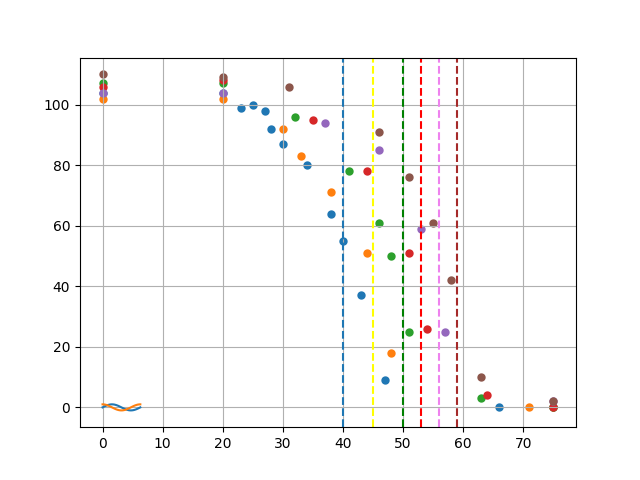
\includegraphics[scale=0.8]{PIC_7.png}\\
\textbf{Рис. 7: } График для определения $B_{\text{кр}}$ в зависимости от $V_a$.
\end{center}

$B_\text{кр}$ будем определять по месту наибольшего углового коэффициента наклона прямой. Делать это достаточно трудно, поэтому абсолютную погрешность его определения будем считать равным $\sigma_{I_m} = 3$ у.е. Пересчитаем $B_\text{кр} = KI_m$, $\varepsilon_{{B_\text{кр}}^2} = 2\varepsilon_{I_m}$. По этим данным построим график. Получаем зависимость $B_{\text{кр}}^2$ от $V_a$.

\begin{center}
\begin{tabular}{|c|c|}
\hline
$B_{\text{кр}}^2$, $\cdot 10^{-6}$ Тл$^2$ & $V_a$, В \\ \hline
20,1 $\pm$ 3,0 & 70 \\ \hline
25,4 $\pm$ 3,4 & 80 \\ \hline
31,4 $\pm$ 3,8 & 90 \\ \hline
35,2 $\pm$ 4,0 & 100 \\ \hline
39,3 $\pm$ 4,2 & 110 \\ \hline
43,7 $\pm$ 4,5 & 120 \\ \hline
\end{tabular}\\
\textbf{Табл. 12:} $B_{\text{кр}}^2$ от $V_a$
\end{center}

		\newpage
	%Страница 11
	
	\begin{flushleft}
		\footnotesize{Определение удельного заряда электрона} \hspace{\fill} \footnotesize{11}
		\\[-0.3cm]\noindent\rule{\textwidth}{0.3pt}
	\end{flushleft}

\begin{center}
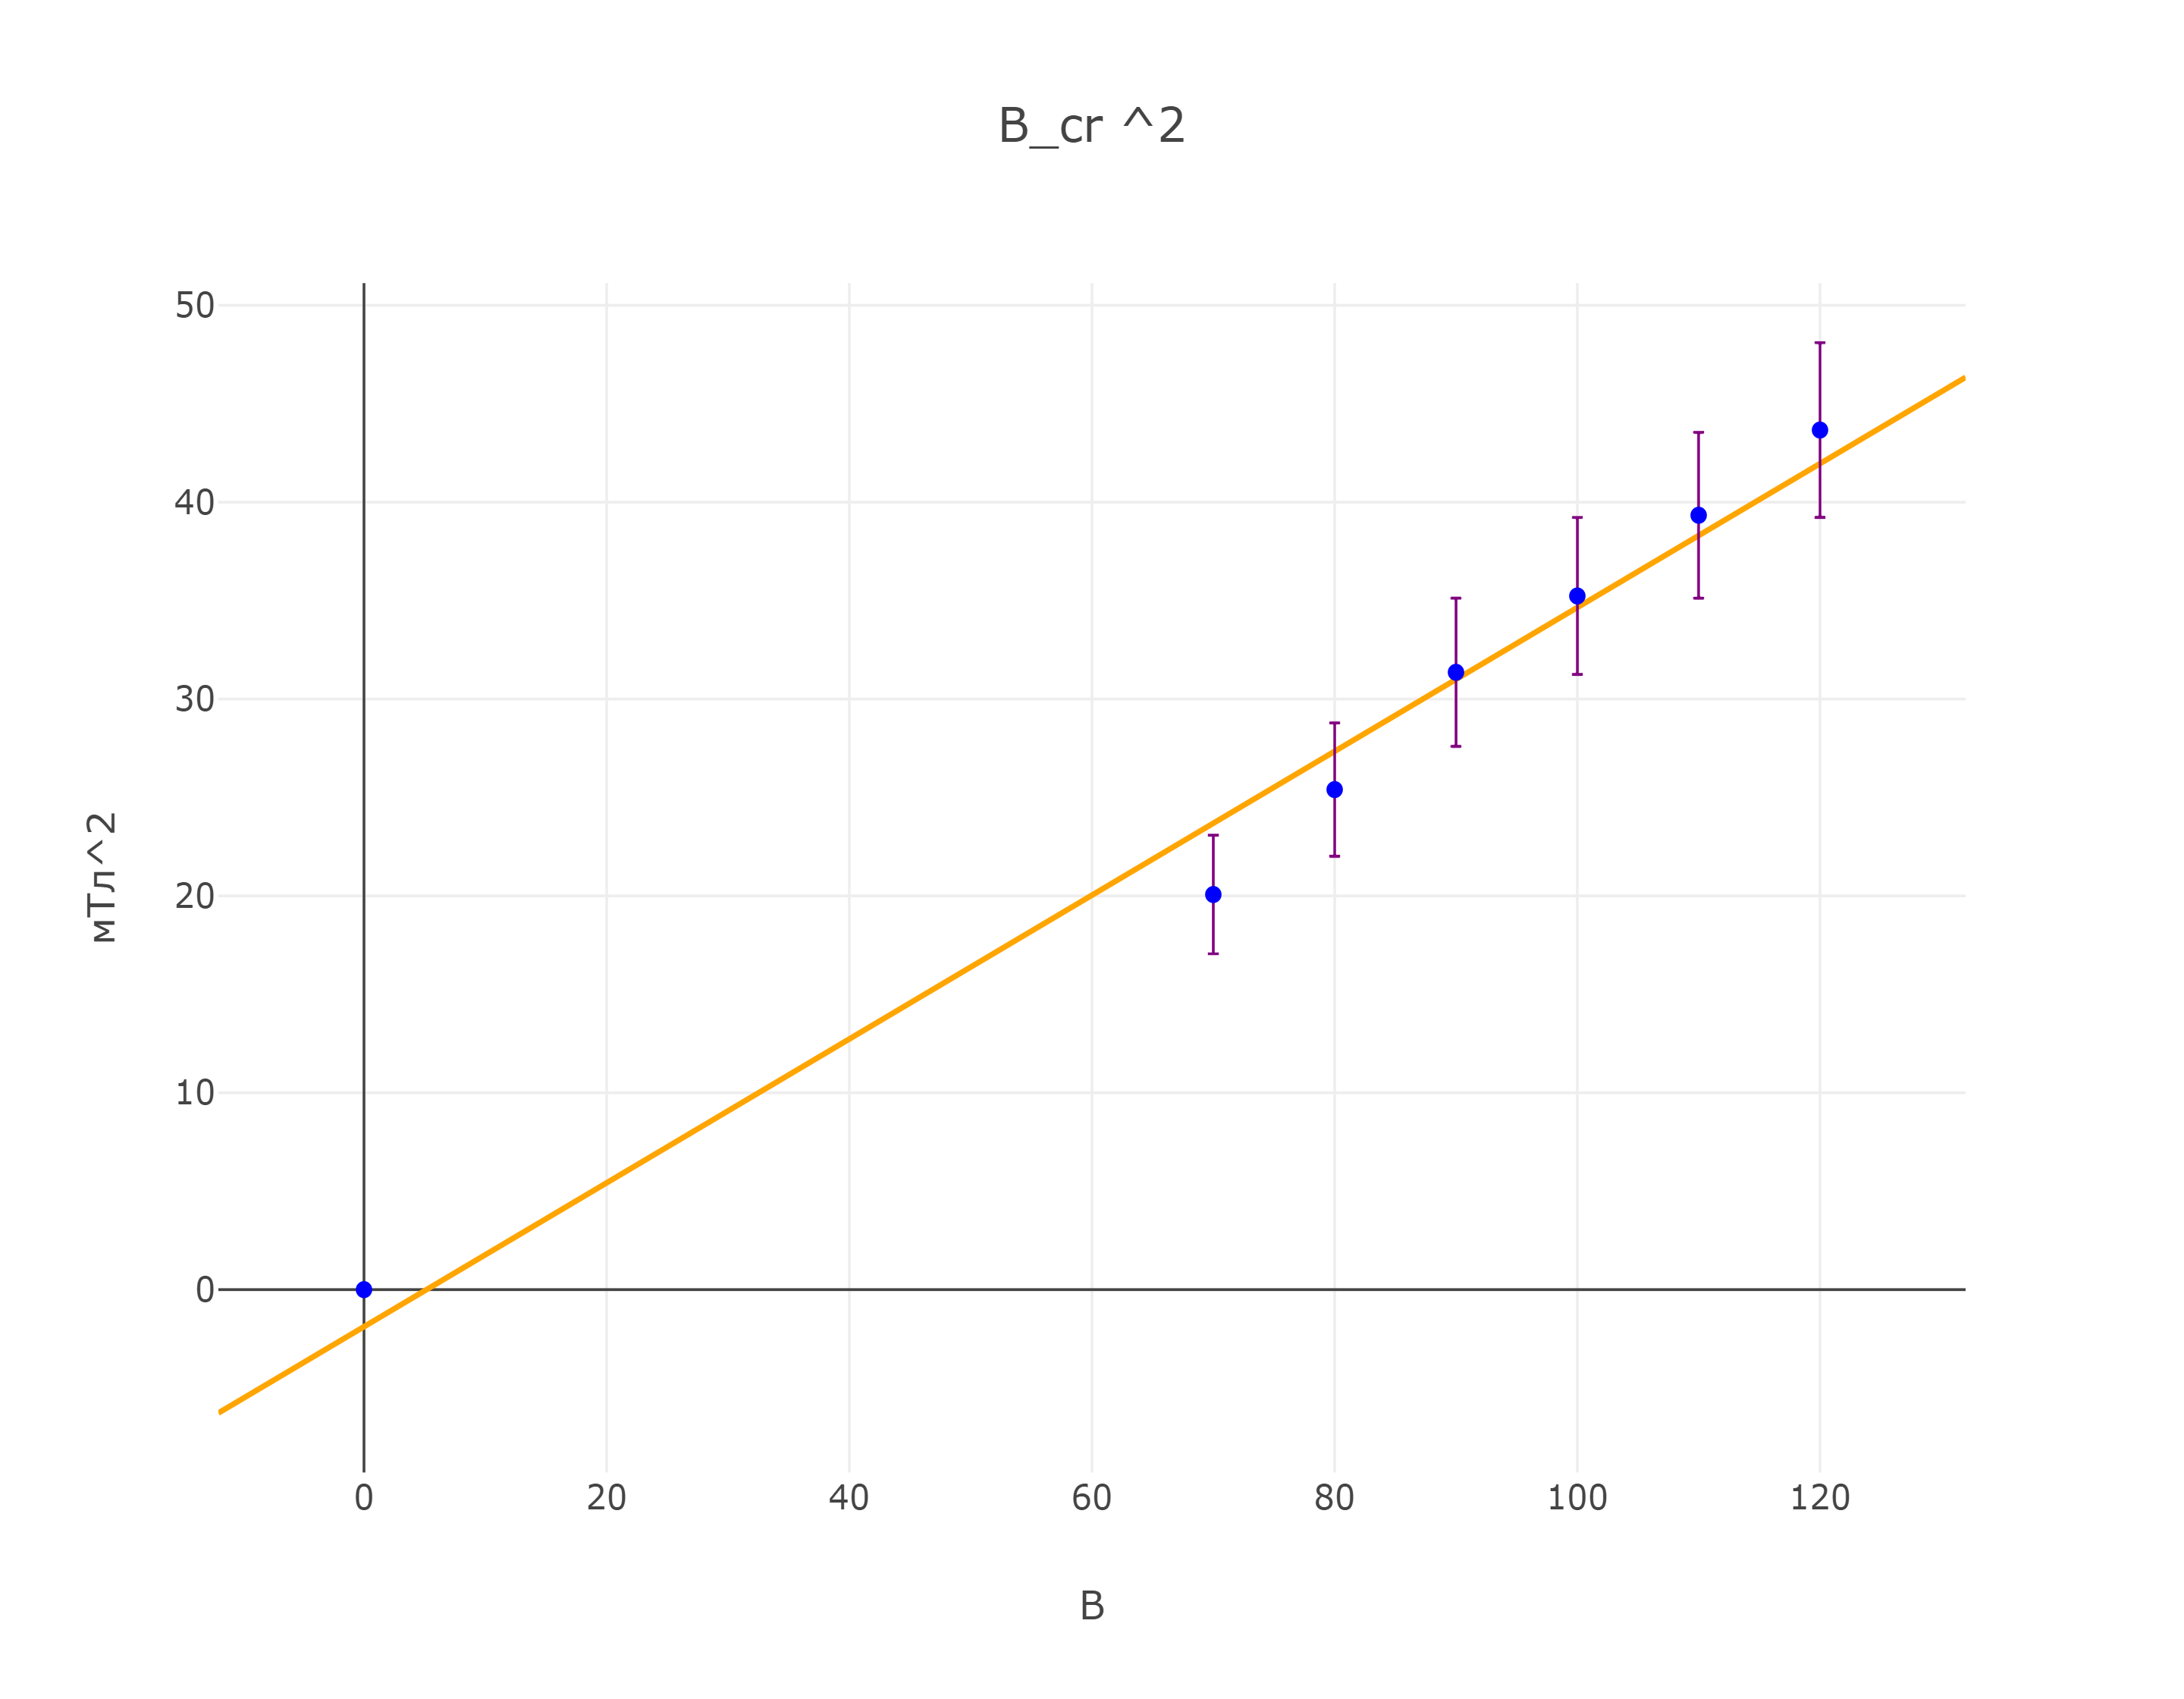
\includegraphics[scale=0.13]{PIC_8.png}\\
\textbf{Рис. 8:} График зависимости $B_{\text{кр}}^2$ от $V_a$.
\end{center}

 По этим данным мы получаем (погрешность углового коэффициента оценена по отклонению от медианной прямой). 
\[\dfrac{e}{m} = (1,5 \pm 0,1) \cdot 10^{11} \text{Кл}/\text{кг}\]

\section{Выводы}

В данной работе мы исследовали зависимость андоного тока от тока, протекающего через соленоид при различных напряжениях на аноде лампы, и по ней рассчитали значение удельного заряда и получили: $e/m = (1,5 \pm 0,1) \cdot 10^{11} \text{Кл}/\text{кг}$. Это значение также близко к табличному $e/m = 1,76 \cdot 10^{11} \text{Кл}/\text{кг}$

\end{document}
